%
% zylinder.tex
%
% (c) 2021 Prof Dr Andreas Müller, OST Ostschweizer Fachhochschule
%
\documentclass[tikz]{standalone}
\usepackage{times}
\usepackage{amsmath}
\usepackage{txfonts}
\usepackage[utf8]{inputenc}
\usepackage{graphics}
\usetikzlibrary{arrows,intersections,math}
\usepackage{ifthen}
\begin{document}

\newboolean{showgrid}
\setboolean{showgrid}{false}
\def\breite{7}
\def\hoehe{4}

\begin{tikzpicture}[>=latex,thick]

% Povray Bild
\node at (0,0) {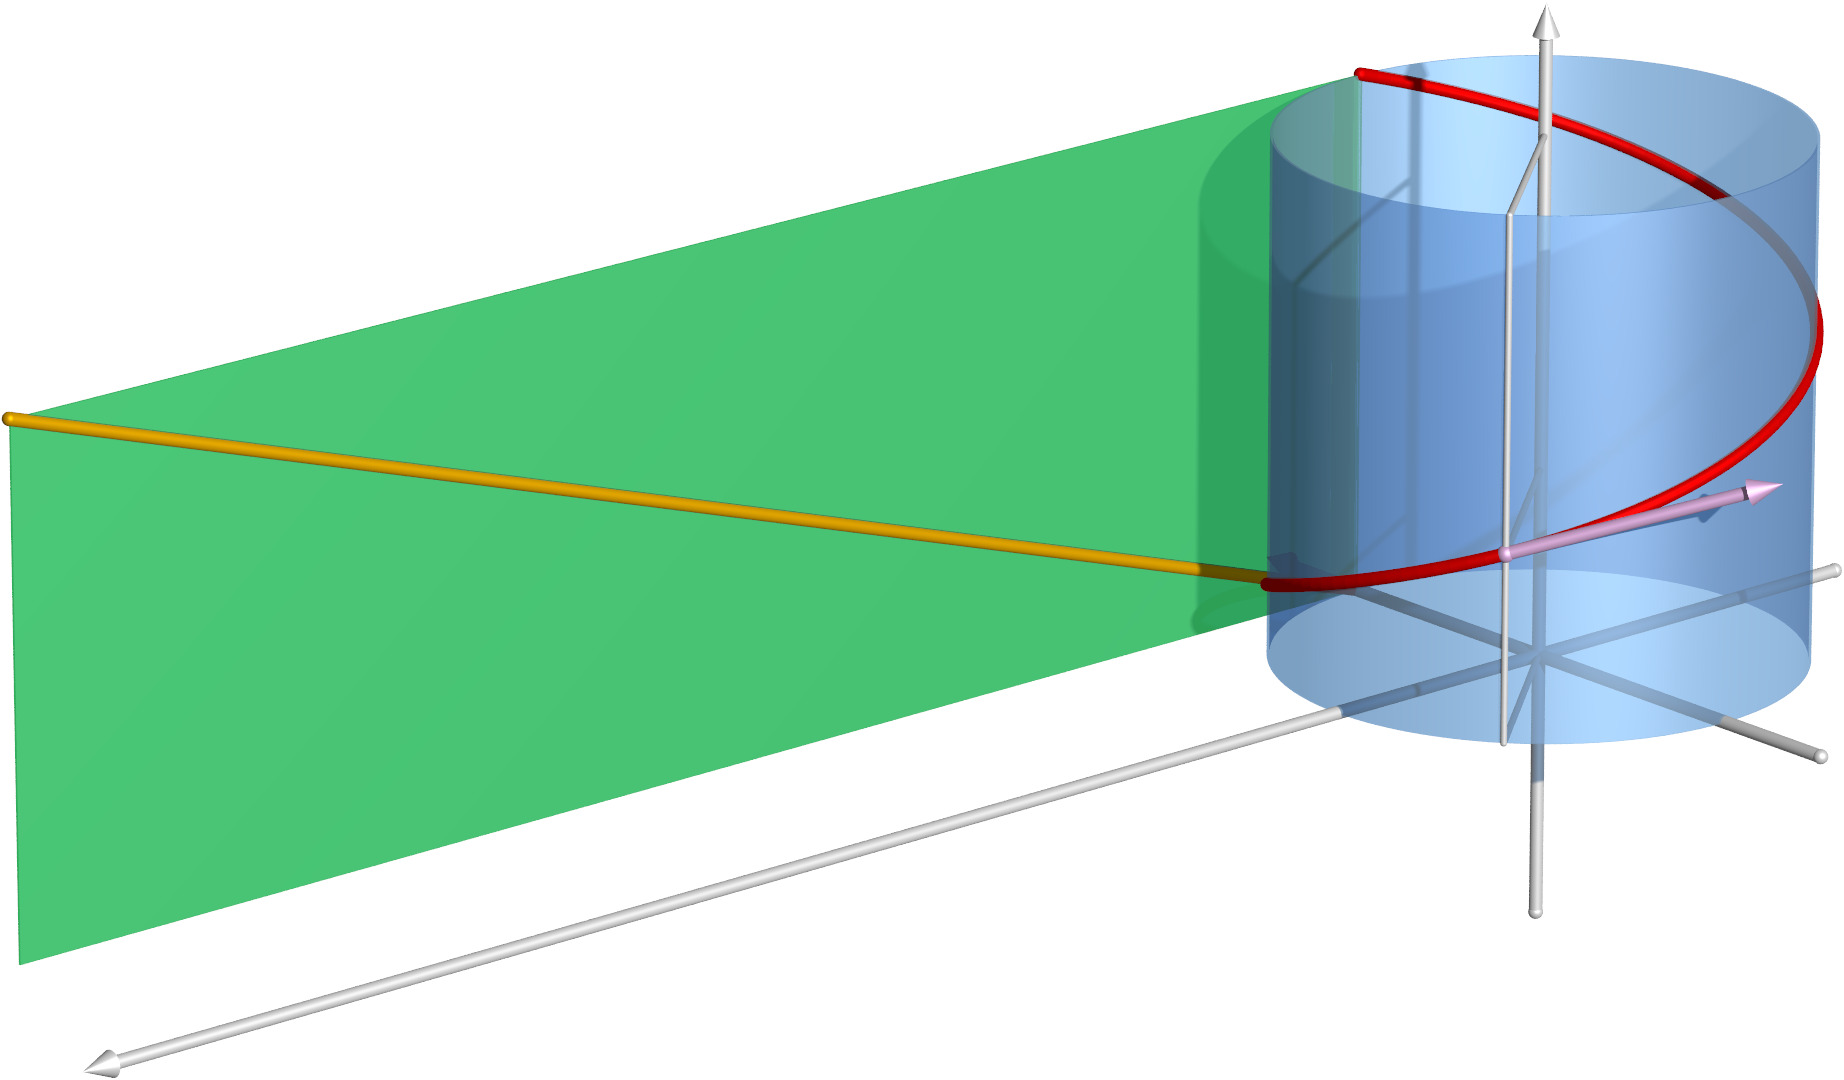
\includegraphics[width=14cm]{zylinder.jpg}};

% Gitter
\ifthenelse{\boolean{showgrid}}{
\draw[step=0.1,line width=0.1pt] (-\breite,-\hoehe) grid (\breite, \hoehe);
\draw[step=0.5,line width=0.4pt] (-\breite,-\hoehe) grid (\breite, \hoehe);
\draw                            (-\breite,-\hoehe) grid (\breite, \hoehe);
\fill (0,0) circle[radius=0.05];
}{}

\node at (-6.4,-3.8) {$y$};
\node at (4.9,4.0) {$z$};
\node at (2.5,0) {$x$};
\node at (-1.8,2.5) [rotate=18] {$2\pi r$};
\node at (-6.9,-1) [left] {$h$};

\node at (4.4,0) [above] {$\gamma(t)$};
\node at (6.5,0.3) [below] {$\dot{\gamma}(t)$};
\node at (4.6,2.6) [above left] {$r$};

\end{tikzpicture}

\end{document}

